\section {Design and Implemenation\\}

\subsection{Reactor Model\\}
The PushUp Server runs atop of the Twisted framework\cite{Twisted}, which is a event-based network programming framework. The highlight of the Twisted is its reactor model\cite{Reactor}.

The reactor is the core of the event loop inside the framework. Event loop is a higher level abstraction of multiplexing model in Linux/Unix (kqueue in Unix and epoll in Linux).

The responsiblities of a event loop is to wait for and dispatches incoming ``events", which will trigger the internal or external "event handlers"(named ``Deferred" in twisted framework, which can be understood as the advanced ``callback" function).

The event loop runs in a single thread and its workflow loop is illustrated in Figure\ref{fig:eventloop}.

\begin{figure}[htb!]
\centering%
    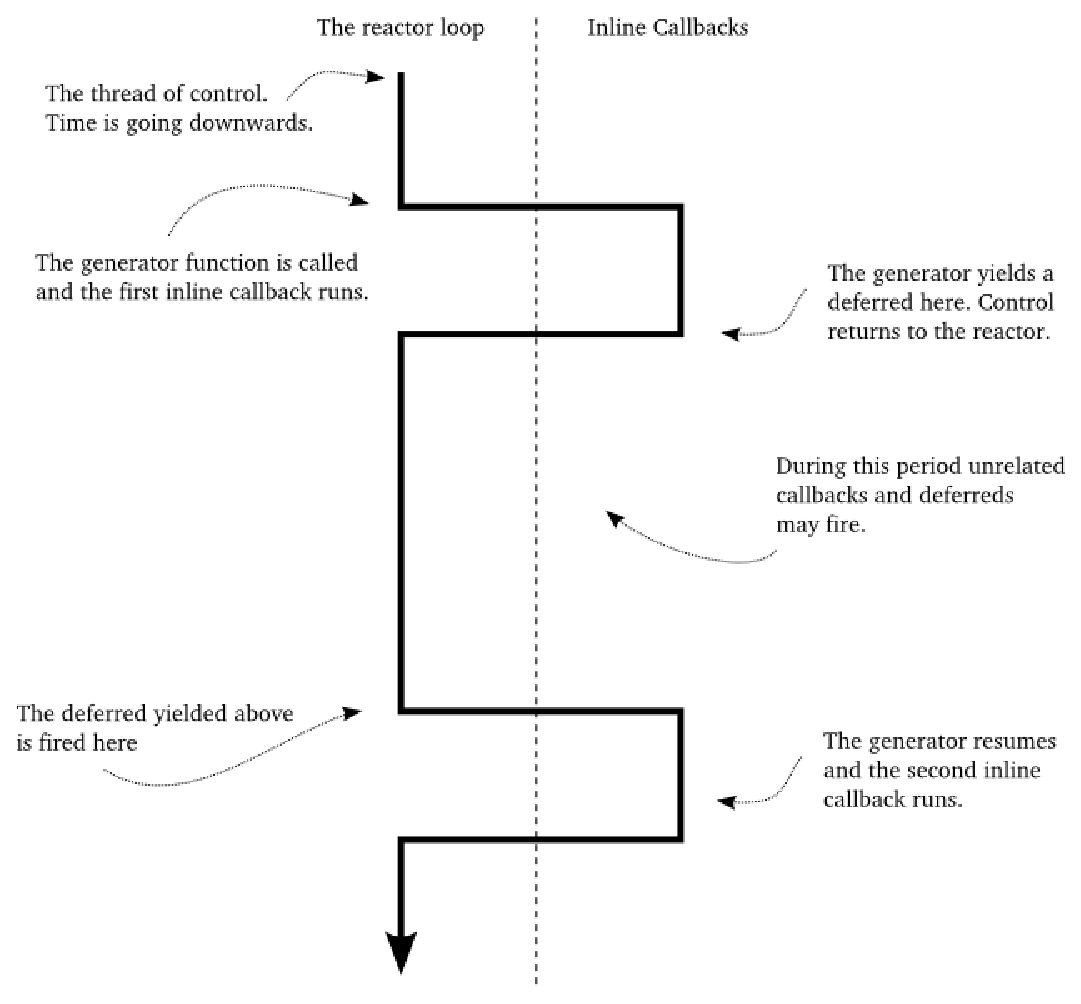
\includegraphics[scale=0.50]{figures/eventloop.eps}
    \caption{Twisted Event Loop}
    \label{fig:eventloop}
\end{figure}


\subsection{Reverse Proxy\\}

How it works, with more details.

\subsection{Message Queue\\}

Pub/Sub: with more details

Publisher: 

    * General design

    * Backend sever connect to the 

Subscriber: 

    * General Design
    * Client Design
    * Just 50 seconds

Message Management

Subscriber

Internal Data structure: what are the highlight of such design.

\subsection{Load Balancer\\}

HAProxy -- based on xxxx.

